\documentclass[20pt]{beamer}
\usepackage{fontspec}
\usepackage{amsfonts}
\usepackage{tangocolors}
\usepackage{listings}
\usepackage{hyperref}
\usepackage{multicol}

\usepackage{tikz}
\usetikzlibrary{shapes}

% thanks http://en.wikibooks.org/wiki/LaTeX/Packages/Listings
\newcommand\normallistingstyle{\lstset{ %
  language=Python,                % the language of the code
  basicstyle=\footnotesize,
                                   % the size of the fonts that are used for the code
  %numbers=left,                   % where to put the line-numbers
  %numberstyle=\tiny\color{gray},  % the style that is used for the line-numbers
  %stepnumber=1,                   % the step between two line-numbers. If it's 1, each line 
                                  % will be numbered
  %numbersep=5pt,                  % how far the line-numbers are from the code
  backgroundcolor=\color{white},      % choose the background color. You must add \usepackage{color}
  showspaces=false,               % show spaces adding particular underscores
  showstringspaces=false,         % underline spaces within strings
  showtabs=false,                 % show tabs within strings adding particular underscores
  %frame=single,                   % adds a frame around the code
  rulecolor=\color{black},        % if not set, the frame-color may be changed on line-breaks within not-black text
  tabsize=2,                      % sets default tabsize to 2 spaces
  %captionpos=b,                   % sets the caption-position to bottom
  breaklines=true,                % sets automatic line breaking
  breakatwhitespace=false,        % sets if automatic breaks should only happen at whitespace
  title=\ ,
  emph={[2]__import__,range,input,raw_input,NameError,dir,dict},
  keywordstyle=\color{ta3chocolate},          % keyword style
  commentstyle=\color{ta3orange},       % comment style
  stringstyle=\color{ta3orange},         % string literal style
  emphstyle={[2]\color{ta2orange}},
  escapeinside=\$\$,            % if you want to add LaTeX within your code
  morekeywords={*,...}               % if you want to add more keywords to the set
  aboveskip=0pt,
  belowskip=0pt,
}}
\newcommand\biglistingstyle{\lstset{ %
    basicstyle=\small,
}}
\newcommand\altlistingstyle{\lstset{ %
    backgroundcolor=\color{black},
    basicstyle=\small\color{white},
    keywordstyle=\color{tachocolate},
    commentstyle=\color{tachameleon},
    stringstyle=\color{tachameleon},
    emphstyle={[2]\color{tabutter}},
    emphstyle={[3]\color{taorange}},
}}
\normallistingstyle
\newcommand\topshade{
    \begin{tikzpicture}[remember picture,overlay]
    \fill[black] (current page.west) rectangle +(100cm, -100cm);
    \end{tikzpicture}
    \vspace{-50pt}
    \biglistingstyle
}
\newcommand\halfshadenopause{
    \altlistingstyle\bigskip\bigskip\bigskip
}
\newcommand\halfshade{
    \pause\halfshadenopause
}
\newcommand\bottomshade{
    \normallistingstyle
}
\newcommand\sk{\par\bigskip\bigskip\par}
\newcommand\wh[1]{\only<#1>{\color{white}}}
\newcommand\tx[2]{\alt<#1>{\textcolor{ta3gray}}{\textcolor{ta3gray}}{\uncover<#1->{#2}}}
\newcommand\rd[2]{\alt<#1>{\textcolor{tagray}}{\textcolor{ta3gray}}{#2}}
%\renewcommand\emph[1]{\textcolor{tagray}{#1}}

\setbeamercolor{itemize item}{fg=ta3gray}
\setbeamercolor{enumerate item}{fg=ta3gray}

\begin{document}
\fontspec[Numbers=Lining]{Open Sans}
\color{ta3gray}

\begin{center}
\title{eval()}
\author{Petr Viktorin}
\date{\today}

\begin{frame}[fragile]
\tiny
\begin{verbatim}
Slides for "Extending FREEIPA", DevConf, Brno, February 2014.

Most of the PDF is just notes that weren't shown on screen

Also used:
  - Apache Directory Studio, connected to ipa33.ipa.test
  - Firefox with these tabs:
    - https://ipa33.ipa.test/       (VM with FreeIPA 3.3)
    - https://ipamaster.ipa.test/   (VM with FreeIPA git master)
    - sozi.svg
    - http://www.zytrax.com/books/ldap/ (unused in the end)
    - http://www.redhat.com/mailman/listinfo/freeipa-devel
    - https://fedorahosted.org/freeipa/report/3
    - http://www.freeipa.org/page/General_considerations
    - http://www.freeipa.org/page/V3_Proposals
    - http://www.freeipa.org/page
        /V3/Multivalued_target_filters_in_permissions
  - terminal with interactive Python for (ipaldap-demo.py)
  - editor with FreeIPA source files mentioned in the PDF
\end{verbatim}
\end{frame}

\frame{\color{ta2gray}
    \sk
    \textbf{EXTENDING FREEIPA}
    \sk\sk
    {Petr Viktorin}\\[-0.25cm]
    {\tiny pviktori@redhat.com}
    \sk
    {\tiny DevConf, 2014-02-08}
}

\frame{
    What is FreeIPA?
}

\frame{
    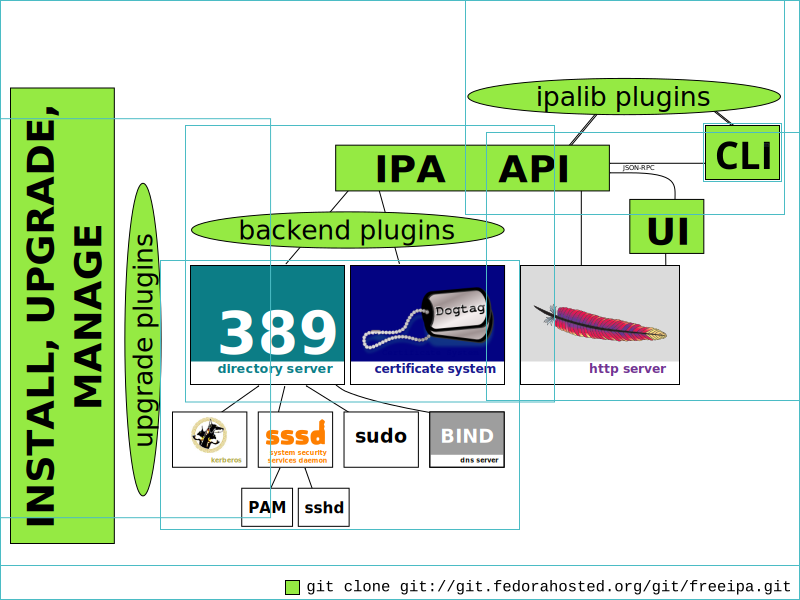
\includegraphics[width=\textwidth]{sozi.pdf}
}

\frame{
    \textbf{LDAP}
    \bigskip\bigskip

    Tree structure

    object classes \& attribute types

    OIDs

    {\small \url{http://www.zytrax.com/books/ldap/}}
}

\frame{
    \textbf{Extending LDAP}
    \bigskip\bigskip

    Schema
        \texttt{\\\tiny install/share/60basev3.ldif}

    \bigskip

    Content updating
        \texttt{\\\tiny install/updates/40-otp.update}

    \bigskip

    ACIs

    \bigskip

    Updater plugins
        \texttt{\\\tiny ipaserver/install/plugins/upload\_cacrt.py}
}

\frame{
    \textbf{ipaldap}
    \bigskip\bigskip

    “Object–LDAP mapper”
    {\tiny\\ see \texttt{ipaldap-demo.py}}
}

\frame{
    \textbf{API plugins}
    \bigskip\bigskip

    Objects \& Methods
    \texttt{\\\tiny ipalib/plugins/user.py}
}

\begin{frame}[fragile]
    \textbf{Objects}
    \bigskip\bigskip

    objectclasses, attributes

    \verb+takes_params+

    attribute name (*?+)

    validators

    \verb+cli_name+

    flags - see \verb+ipalib.parameters.Param+

    default permissions
\end{frame}

\begin{frame}[fragile]
    \textbf{Methods}
    \bigskip\bigskip

    run

    forward

    execute
\end{frame}

\begin{frame}[fragile]
    \textbf{Callbacks}
    \bigskip\bigskip

    \tiny
    \begin{itemize}
    \item[]
    \verb+pre_callback+\\
    Extra validation, generating random password

    \item[]
    \verb+post_callback+\\
    Updating other entries, tweaking output

    \item[]
    \verb+exc_callback+\\
    Error handling

    \item[]
    \verb+interactive_prompt_callback+\\
    Prompting for values
    \end{itemize}
\end{frame}

\begin{frame}[fragile]
    \textbf{\phantom{”}Other “plugins”}
    \bigskip\bigskip

    DS plugins

    UI facets

    Tests
\end{frame}

\section{EXTENDING FREEIPA}
\begin{frame}[fragile]
    \textbf{EXTENDING FREEIPA}
\end{frame}

\begin{frame}[fragile]
    \textbf{A. Extend the core}

    \bigskip

    \begin{itemize}
    \item[$+$] tweak everything
    \item[$-$] gotta play by the rules
    \end{itemize}

    \bigskip\bigskip

    \textbf{B. External plugin}

    \bigskip

    \begin{itemize}
    \item[$+$] do whatever you want
    \item[$-$] hic sunt leones
    \end{itemize}
\end{frame}

\begin{frame}[fragile]
    \textbf{A. Extend the core}
    \bigskip\bigskip

    \begin{enumerate}
    \item \href{www.redhat.com/mailman/listinfo/freeipa-devel}{Say hello}
    \item \href{https://fedorahosted.org/freeipa/report/3}{File an RFE ticket}
    \item \href{http://www.freeipa.org/page/General_considerations}{Read General Considerations}
    \item \href{http://www.freeipa.org/page/V3_Proposals}{Write a Design page}
    \item Submit patches
    \item Profit!
    \end{enumerate}
\end{frame}

\begin{frame}[fragile]
    \textbf{B. External plugin}
    \bigskip\bigskip

    \begin{enumerate}
    \item Say hello!
    \item Write a plugin
    \item Share the plugin
    \item Package the plugin
    \item Profit!
    \end{enumerate}
\end{frame}

\frame{

    \bigskip\bigskip
    \bigskip\bigskip
    \bigskip\bigskip

    {\huge ?}

    \bigskip\bigskip
    \bigskip\bigskip
    \bigskip\bigskip
    \bigskip\bigskip
}
% 
% \frame{
%     \small
%     \rd{1}{Sources} \& links\\[0.25cm]
%     \bigskip\bigskip
%     \tiny
%     \tx{1}{\href{http://www.python.org/dev/peps/pep-3156/}{PEP 3156 - Asynchronous IO Support Rebooted: the "asyncio" Module}}\\[0.25cm]
%     \tx{1}{\href{http://www.python.org/dev/peps/pep-3148/}{PEP 3148 - futures - execute computations asynchronously}}\\[0.25cm]
%     \tx{1}{\href{http://www.python.org/dev/peps/pep-3153/}{PEP 3153 (Superseded) - Asynchronous IO support}}\\[0.25cm]
%     \tx{1}{\url{http://docs.python.org/3.4/library/asyncio.html}}\\[0.25cm]
%     \tx{1}{\href{http://www.youtube.com/watch?v=1coLC-MUCJc}{Youtube: Guido van Rossum - Tulip: Async I/O for Python 3}}\\[0.25cm]
%     %\bigskip
%     %\tx{1}{\url{}}\\[0.25cm]
%     %\tx{1}{\url{}}\\[0.25cm]
%     %\tx{1}{\url{}}\\[0.25cm]
%     %\tx{1}{\url{}}\\[0.25cm]
%    
% }
% 
\end{center}
\end{document}

